\addchap{Wichtige Gebäude auf dem Campus}

Auch wenn der Eine oder Andere sich das vielleicht wünscht, wird sich nicht das gesamte Studium in einem Gebäude abspielen.
Stattdessen gibt es einige wichtige Gebäude, die in deinem Studienalltag eine Rolle spielen werden.

\begin{figure}[b!]
    \centering
    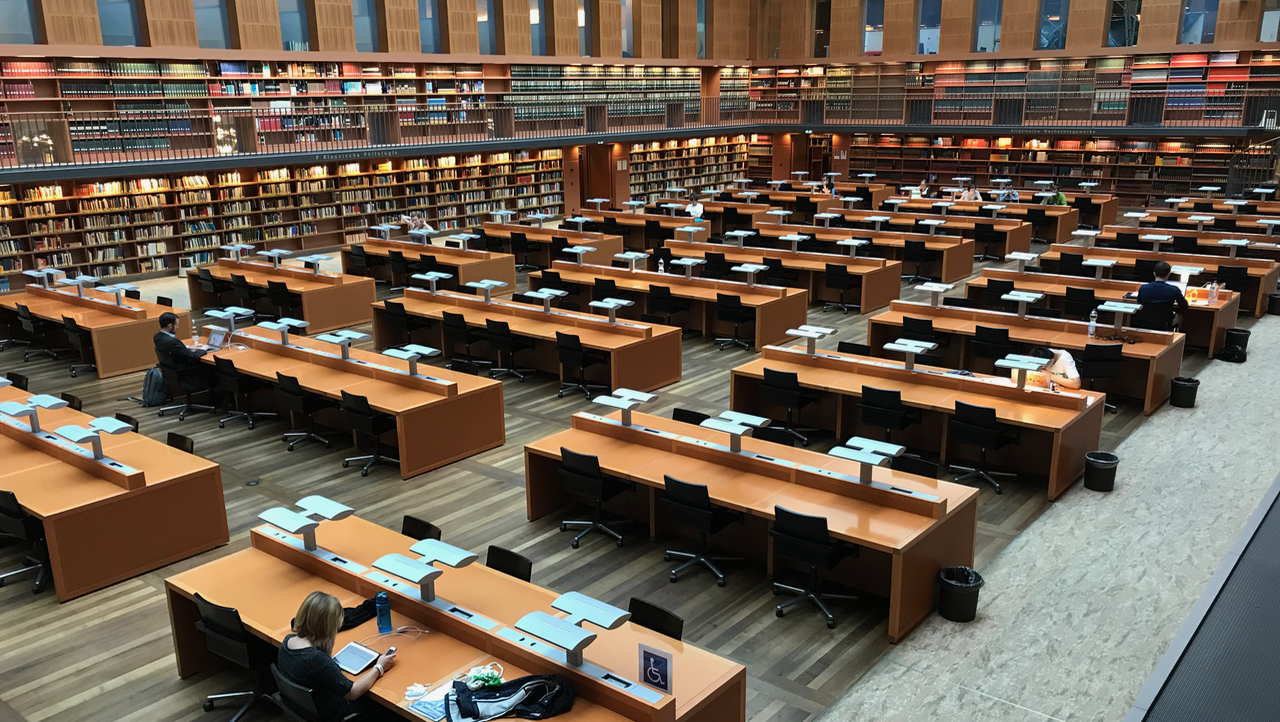
\includegraphics[width=\linewidth]{img/slub-lesesaal}
\end{figure}

\minisec{SLUB}

Die Sächsische Landesbibliothek – Staats- und Universitätsbibliothek Dresden, kurz \emph{SLUB} ist das, was an anderen Universitäten einfach Bib heißt.
Mit einer Auswahl von über 12 Millionen Bestandseinheiten bestehend aus Büchern, Magazinen, Filmen, etc.\ ist sie eine der größten (Universitäts-)Bibliotheken Deutschlands.
Wer denkt, für ein erfolgreiches Informatikstudium nie ein Buch in die Hand nehmen zu müssen, liegt jedoch komplett richtig, denn dafür bietet die SLUB auch eine umfangreiche Auswahl online verfügbarer Ressourcen, die ihr euch als Studierende kostenfrei herunterladen könnt.
Doch auch für notorische Nicht-Leser ist die SLUB ein beliebter Aufenthaltsort unter Studierenden, besonders wegen der vielen ruhigen Arbeitsplätze, die im Gebäude zur Verfügung stehen.
Wollt ihr mit Anderen gemeinsam lernen, gibt es dafür einen weiträumigen Eingangsbereich mit Gruppentischen.
Darüber hinaus können private Gruppenräume reserviert werden. Ein schönes Café, in dem per Mensakarte bezahlt werden kann, rundet das Ganze ab.
Vom APB aus befindet sich die Bibliothek jedoch am anderen Ende des Campus, was aber für Studienanfänger oft kein Problem darstellt.

\minisec{HSZ}

Denn gerade die Grundlagenvorlesungen finden nicht im APB, sondern im Hörsalzentrum (\emph{HSZ}) statt.
In diesem, im Vergleich zum APB doch sehr eintönigen Gebäude werdet ihr viele Vorlesungen zu den Grundlagen der Informatik erleben und beim Pendeln zwischen APB und HSZ den einen oder anderen Kilometer ansammeln.
Das HSZ umfasst vier Vorlesungssäle, unter Anderem das Audimax, den größten Hörsaal der Universität und das größte Auditorium Sachsens.
Zusätzlich finden sich hier noch einige Seminarräume, in welchen Übungen stattfinden können. Vor dem "zentralen Kubus" steht meist ein Mensawagen für den kleinen Hunger zwischendurch.
Auf der anderen Seite des Gebäudes ist die schöne Wiese des HSZ Veranstaltungsort für Feste oder Messen.
Zudem findet ihr dort den Grillcube, der euch für die Pausen zwischen Vorlesungen mit Burgern versorgt.

\minisec{Mensen}
Wer sein Studium nicht mit Pizzabestellungen bestreiten will, muss das zum Glück auch nicht, denn das Studentenwerk betreibt ein Netz aus 18 Mensen.
Egal in welchem Gebäude der Universität ihr euch befindet, in der Nähe wird eine Mensa oder zumindest ein Café zu finden sein.
Die größte der Mensen, die Alte Mensa, befindet sich glücklicherweise direkt zwischen Fakultät und HSZ.
Hier findet ihr eine Vielzahl an täglich wechselnden Hauptgerichten, Salaten und Nachspeisen.
Das Tagesangebot aller Mensen ist auf der Seite des Studierendenwerks \link{https://www.studentenwerk-dresden.de/mensen/speiseplan/} zu finden.
Für Freunde des späten Frühstücks, oder Studierende mit gestörtem Schlafrhythmus findet sich in der Alten Mensa Mo-Do bis 20 Uhr ein warmes Abendangebot. Die Auswahl ist jedoch nach 15 Uhr zunehmend eingeschränkter.
Da die Mensa zu Stoßzeiten der Fülle an Menschen kaum standhalten kann, bieten sich Essenszeiten an, die NICHT direkt nach Ende einer Doppelstunde beginnen.
Auch am Wochenende könnt ihr dem Kochen entkommen, denn der Siedepunkt hat auch an Samstagen und Sonntagen geöffnet.
Gerade nach einer produktiven Lerneinheit in der SLUB ist diese ganz bequem mit einem einfachen Wechsel der Straßenseite zu erreichen.

\minisec{Seminargebäude}

In diesem Bau, an der besonders schönen Fassade erkennbar, finden die Sprachkurse des LSK statt.
Für alle, die über einen einfachen Sprachkurs hinausgehen wollen, werden zusätzlich Seminare zur Kultur und Politik ausgewählter Länder und Regionen angeboten.
Weitere Informationen findet ihr auf der Website des LSK \link{https://tu-dresden.de/gsw/slk/lsk}.
Das Gebäude steht direkt neben der SLUB, ca. 20 Minuten vom APB entfernt.
